\documentclass[a4paper,11pt]{article}
\usepackage{tikz}
\usetikzlibrary{shapes}
\usepackage{fullpage}

\input{macros}

\newcommand{\Timeout}{600.00} % CPU seconds
\definecolor{fields}{HTML}{FFDF42}
\definecolor{forrest}{HTML}{3C8031}
\definecolor{pasture}{HTML}{7FFF00}
\definecolor{mountain}{HTML}{949698}
\definecolor{hills}{HTML}{F26035}
\definecolor{desert}{HTML}{FBB982}

\title{\textbf{Generating a "fair" \\
    Settlers of Catan game board layout using \\
    Constraint Programming
  }
}

\author{Frej Knutar} % replace by your name(s)

%\date{Month Day, Year}
\date{\today}

\begin{document}

\maketitle

\section{Settlers of Catan}

\subsection{Game introduction}
\label{sec:introduction}
Settlers of Catan\cite{settlers} is a multi-player board game that is played on a board consisting of 19 hexagon terrain pieces. Each terrain piece has one of 6 terrain \textit{piece types} and on top of each an \textit{allotment number} is placed, except if the terrain type is the desert terrain type, then the terrain piece has no allotment number placed on top of it. The allotment numbers represent what result a pair of six-sided dies needs to show in order for that field to yield a resource corresponding to it. The terrain piece types are fields, forest, pasture, mountains, hills, and desert, yielding the resources grain, wood, wool, ore, brick, and nothing respectively. During the game the players can place \textit{settlements}. Placing settlements is one of the main ways of the players to advance the game in their favor. The settlements are placed on \textit{junctions}. Junctions are where two or three terrain pieces meet at the edges of those terrain piece hexagons. Given that that the allotment number of a terrain piece is shown on the dies, then each player that has one or more settlements on edge on the terrain piece receives one resource of the appropriate for each such settlement.

\subsection{Game board fairness}
\label{sec:boardFairness}
The placement of the allotment numbers and the terrain pieces greatly dictate what junctions and terrain types that are considered \textit{profitable} and \textit{unprofitable}. It is considered profitable to place settlements in junctions with high \textit{scoring} allotment values. The score of an allotment number is how likely it is that two six-sided dies shows the allotment number.

\subsubsection{Junction fairness}
\label{sec:junctionFairness}
The score of a junction the board can be described as the sum over all the scores of the allotment numbers in that junction. The overall fairness of the allotment numbers of the junctions can then be said to be the difference between a highest scoring junction compared to a lowest scoring junction, where only junctions with three terrain pieces are compared. A small difference indicates that the allotment numbers have a good distribution over the junctions of the board, while a big difference indicates that they have not.

\subsubsection{Terrain type fairness}
\label{sec:typeFairness}
The allotment score of a terrain type $t$~can be described as the mean of the of the allotment number scores of all the terrain pieces of type $t$. Similarly to when scoring junctions, the overall fairness of the allotment numbers of the terrain types can be said to be the difference between a highest mean of the terrain types compared to a lowest mean of the terrain types. A small difference indicates that the allotment numbers have a good distribution over the terrain types, while a big difference indicates that they have not.

\subsubsection{Harbours}
\label{sec:harbours}
Some junctions on the board are considered to be \textit{harbours}. Some of these harbours have a resource type associated with it, and terrain pieces with the corresponding resource type may not be placed so the harbour is a junction of that tile.

\subsection{Game board layout requests}
\label{sec:requests}
Some requests of players have helped stating constraints that either make the game more balanced or make the game more fun for those players. One such constraint is that each terrain piece may not have any neighbouring terrain pieces with the same type as itself. Another request was that 3 the 6 most centric allotment numbers must be either 8 or 6.

\begin{figure}
\label{figure:bestmatch}
\begin{center}
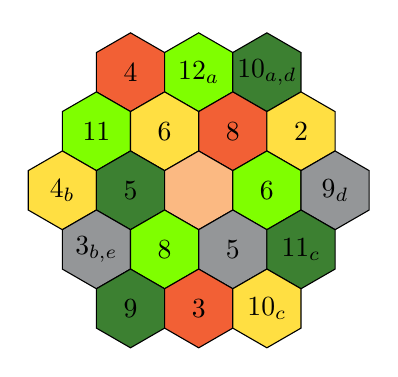
\begin{tikzpicture} [hexa/.style= {shape=regular polygon,regular polygon sides=6,minimum size=1cm, draw,inner sep=0,anchor=south,fill=lightgray!85!blue,rotate=30}]
  % Row 1
  {\node[hexa] [fill=hills]    (1;2) at ({1*sin(60)},0) { };}
  {\node[hexa] [fill=pasture]  (1;3) at ({2*sin(60)},0) { };}
  {\node[hexa] [fill=forrest]  (1;4) at ({3*sin(60)},0) { };}
  % Row 2
  {\node[hexa] [fill=pasture]  (2;1) at ({0.5*sin(60)},-0.75) { };}
  {\node[hexa] [fill=fields]   (2;2) at ({1.5*sin(60)},-0.75) { };}
  {\node[hexa] [fill=hills]    (2;3) at ({2.5*sin(60)},-0.75) { };}
  {\node[hexa] [fill=fields]   (2;4) at ({3.5*sin(60)},-0.75) { };}
  % Row 3
  {\node[hexa] [fill=fields]   (3;1) at (0,-1.5) { };}
  {\node[hexa] [fill=forrest]  (3;2) at ({1*sin(60)},-1.5) { };}
  {\node[hexa] [fill=desert]   (3;3) at ({2*sin(60)},-1.5) { };}
  {\node[hexa] [fill=pasture]  (3;4) at ({3*sin(60)},-1.5) { };}
  {\node[hexa] [fill=mountain] (3;5) at ({4*sin(60)},-1.5) { };}
  % Row 4
  {\node[hexa] [fill=mountain] (4;1) at ({0.5*sin(60)},-2.25) { };}
  {\node[hexa] [fill=pasture]  (4;2) at ({1.5*sin(60)},-2.25) { };}
  {\node[hexa] [fill=mountain] (4;3) at ({2.5*sin(60)},-2.25) { };}
  {\node[hexa] [fill=forrest]  (4;4) at ({3.5*sin(60)},-2.25) { };}
  % Row 5
  {\node[hexa] [fill=forrest] (5;2) at ({1*sin(60)},-3) { };}
  {\node[hexa] [fill=hills]   (5;3) at ({2*sin(60)},-3) { };}
  {\node[hexa] [fill=fields]  (5;4) at ({3*sin(60)},-3) { };}
  %Row 1
  {\node [circle] at (1;2) {$4$};}
  {\node [circle] at (1;3) {$12_a$};}
  {\node [circle] at (1;4) {$10_{a,d}$};}
  %Row 2
  {\node [circle] at (2;1) {$11$};}
  {\node [circle] at (2;2) {$6$};}
  {\node [circle] at (2;3) {$8$};}
  {\node [circle] at (2;4) {$2$};}
  %Row 3
  {\node [circle] at (3;1) {$4_b$};}
  {\node [circle] at (3;2) {$5$};}
  {\node [circle] at (3;4) {$6$};}
  {\node [circle] at (3;5) {$9_d$};}
  %Row 4
  {\node [circle] at (4;1) {$3_{b,e}$};}
  {\node [circle] at (4;2) {$8$};}
  {\node [circle] at (4;3) {$5$};}
  {\node [circle] at (4;4) {$11_c$};}
  %Row 5
  {\node [circle] at (5;2) {$9$};}
  {\node [circle] at (5;3) {$3$};}
  {\node [circle] at (5;4) {$10_c$};}
\end{tikzpicture}
\end{center}
\caption{An example of a Settlers of Catan board setup, and a solution to the COP. The gold yellow, dark green, light green, dark gray, orange, and light brown terrain pieces are fields, forest, pasture, mountains, hills and desert respectively. The subscript notation of the board pieces with characters $a$, $b$, $c$, $d$, and $e$ indicates that those pieces are resource harbours and that pieces of piece types fields, forest, pasture, mountains, and hills cannot be placed on those respectively.}
\end{figure}

\section{Model}
\label{sec:model}
This section will give a constraint optimisation model (COP) of the Settlers of Catan game board fairness problem. In this problem the desert terrain piece is always placed in the centre of the board; on row 3 and column 3. The desert terrain piece is considered to be not active.

\begin{figure}
\label{figure:layout}
\begin{center}
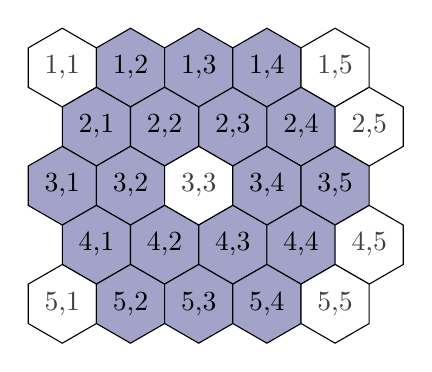
\begin{tikzpicture} [hexa/.style= {shape=regular polygon,regular polygon sides=6,minimum size=1cm, draw,inner sep=0,anchor=south,fill=lightgray!85!blue,rotate=30}]
  % Row 1
  {\node[hexa][fill=white] (1;1) at (0,0) { };}
  {\node[hexa] (1;2) at ({1*sin(60)},0) { };}
  {\node[hexa] (1;3) at ({2*sin(60)},0) { };}
  {\node[hexa] (1;4) at ({3*sin(60)},0) { };}
  {\node[hexa][fill=white] (1;5) at ({4*sin(60)},0) { };}
  % Row 2
  {\node[hexa] (2;1) at ({0.5*sin(60)},-0.75) { };}
  {\node[hexa] (2;2) at ({1.5*sin(60)},-0.75) { };}
  {\node[hexa] (2;3) at ({2.5*sin(60)},-0.75) { };}
  {\node[hexa] (2;4) at ({3.5*sin(60)},-0.75) { };}
  {\node[hexa][fill=white] (2;5) at ({4.5*sin(60)},-0.75) { };}
  % Row 3
  {\node[hexa] (3;1) at (0,-1.5) { };}
  {\node[hexa] (3;2) at ({1*sin(60)},-1.5) { };}
  {\node[hexa][fill=white] (3;3) at ({2*sin(60)},-1.5) { };}
  {\node[hexa] (3;4) at ({3*sin(60)},-1.5) { };}
  {\node[hexa] (3;5) at ({4*sin(60)},-1.5) { };}
  % Row 4
  {\node[hexa] (4;1) at ({0.5*sin(60)},-2.25) { };}
  {\node[hexa] (4;2) at ({1.5*sin(60)},-2.25) { };}
  {\node[hexa] (4;3) at ({2.5*sin(60)},-2.25) { };}
  {\node[hexa] (4;4) at ({3.5*sin(60)},-2.25) { };}
  {\node[hexa][fill=white] (4;5) at ({4.5*sin(60)},-2.25) { };}
  % Row 5
  {\node[hexa][fill=white] (5;1) at (0,-3) { };}
  {\node[hexa] (5;2) at ({1*sin(60)},-3) { };}
  {\node[hexa] (5;3) at ({2*sin(60)},-3) { };}
  {\node[hexa] (5;4) at ({3*sin(60)},-3) { };}
  {\node[hexa][fill=white] (5;5) at ({4*sin(60)},-3) { };}
  %Row 1
  {\node [circle,darkgray] at (1;1) {1,1};}
  {\node [circle] at (1;2) {1,2};}
  {\node [circle] at (1;3) {1,3};}
  {\node [circle] at (1;4) {1,4};}
  {\node [circle,darkgray] at (1;5) {1,5};}
  %Row 2
  {\node [circle] at (2;1) {2,1};}
  {\node [circle] at (2;2) {2,2};}
  {\node [circle] at (2;3) {2,3};}
  {\node [circle] at (2;4) {2,4};}
  {\node [circle,darkgray] at (2;5) {2,5};}
  %Row 3
  {\node [circle] at (3;1) {3,1};}
  {\node [circle] at (3;2) {3,2};}
  {\node [circle,darkgray] at (3;3) {3,3};}
  {\node [circle] at (3;4) {3,4};}
  {\node [circle] at (3;5) {3,5};}
  %Row 4
  {\node [circle] at (4;1) {4,1};}
  {\node [circle] at (4;2) {4,2};}
  {\node [circle] at (4;3) {4,3};}
  {\node [circle] at (4;4) {4,4};}
  {\node [circle,darkgray] at (4;5) {4,5};}
  %Row 5
  {\node [circle,darkgray] at (5;1) {5,1};}
  {\node [circle] at (5;2) {5,2};}
  {\node [circle] at (5;3) {5,3};}
  {\node [circle] at (5;4) {5,4};}
  {\node [circle,darkgray] at (5;5) {5,5};}
\end{tikzpicture}
\caption{The hexagon tiles. The blue tiles are the active tiles of the board, while the white are the non-active tiles. The pair of numbers on each tile represents that tiles row and column position respectively. In this model the desert tile is considered to not be active.}
\end{center}
\end{figure}

\newcommand{\Rows}{\textit{rows}}
\newcommand{\Cols}{\textit{columns}}
\newcommand{\PieceTypes}{\textit{pieceTypes}}
\newcommand{\PieceTypesCounts}{\textit{pieceCounts}}
\newcommand{\AllotmentNumberValues}{\textit{allotmentNumberValues}}
\newcommand{\AllotmentNumberScores}{\textit{allotmentNumberScores}}
\newcommand{\AllotmentNumberCounts}{\textit{allotmentNumberCounts}}
\newcommand{\ActivePieces}{\textit{activePieces}}
\newcommand{\Junctions}{\textit{junctions}}
\newcommand{\Harbours}{\textit{harbours}}

\subsection{Data and Derived Constants}
\begin{itemize}
\item \Rows~designates the ordered array of row indices $[1,2,\dots,5]$.

\item \Cols~designates the ordered array of column indices $[1,2,\dots,5]$.

\item \PieceTypes~designates the ordered array of the different board piece types. The different board pieces are fields, forest, pasture, mountain, hills, and desert, corresponding to the integers $1$, $2$, $3$, $4$, $5$, and $6$ respectively. Hence $\PieceTypes=[1,2,3,4,5,6]$

\item \PieceTypesCounts~designates the number of instances of each terrain piece type. There exist $\PieceTypesCounts[f]$ piece types of terrain piece type $f \in \PieceTypes$. Here $\PieceTypesCounts = [4,4,4,3,3,1]$.

\item \AllotmentNumberValues~designates the values that the allotment numbers can take, here the ordered array $[2,\dots,6,8,\dots,12]$. Note that $7$ is \textbf{not} an allotment number.

\item \AllotmentNumberScores~designates the scores of the allotment numbers, here the ordered array $[\frac{1}{36},\frac{2}{36}\dots,\frac{5}{36},\frac{5}{36},\frac{4}{36}\dots,\frac{1}{36}]$, \\ hence $\Cardinality{\AllotmentNumberValues} = \Cardinality{\AllotmentNumberScores} = 10$. 

\item \AllotmentNumberCounts~designates the number of instances for each allotment number. There are $\AllotmentNumberCounts[i]$ allotment numbers for allotment number value $a = \AllotmentNumberValues[i]$, hence $\Cardinality{\AllotmentNumberValues} = \Cardinality{\AllotmentNumberCounts} = 10$. Here $\AllotmentNumberCounts = [1,2,2,2,2,2,2,2,2,1]$.

\item \ActivePieces~designates the two dimensional indicating if game board pieces are considered active or not. Given $a = \ActivePieces[r][c], r \in \Rows, c \in \Cols$, then a game board piece must be placed on the board on row $r$ and column $c$ if $a=1$, otherwise $a = 0$ and a terrain piece cannot be placed on row $r$ column $c$. Hence $\ActivePieces[r,c] \in \Set{0,1}$. The active pieces can be seen in \ref{figure:layout}.

\item $\Junctions$ designates the ordered array holding the junctions on the board where three active terrain pieces intersect. Each junction holds a set of three board positions \\ $\Set{ \Tuple{r_1,c_1}, \Tuple{r_2,c_2}, \Tuple{r_3,c_3} }$, where $r_i \in \Rows, c_i \in \Cols, i \in \Set{1,2,3}$.

\item $harbours$ designates the terrain piece locations that are considered resource harbours on the board. There are five harbours, one for each resource type, and each occupy two adjacent tiles.

\end{itemize}

\newcommand{\Pieces}{\textit{pieces}}
\newcommand{\AllotmentNumbers}{\textit{allotmentNumbers}}
\newcommand{\AllotmentScores}{\textit{allotmentScores}}
\newcommand{\JunctionScores}{\textit{junctionScores}}
\newcommand{\PieceTypeScoreMean}{\textit{PieceTypeScoreMean}}

\subsubsection{Decision Variables}
\begin{itemize}
\item $\Pieces$ designates the ordered array of terrain piece types of the board. If the piece in row $r \in \Rows$ and column $c \in \Cols$ is active, $\ActivePieces[r,c]=1$, then $\Pieces[r,c] \in \PieceTypes$, else the piece is not active, $\ActivePieces[r,c]=0$, and $\Pieces[r,c] = 0$

\item $\AllotmentNumbers$ designates the allotment numbers of the terrain pieces. If the piece in row $r \in \Rows$ and column $c \in \Cols$ is active, $\ActivePieces[r,c]=1$, then \\
$\AllotmentNumbers[r,c] \in \AllotmentNumberValues$, else the piece is not active, \\
$\ActivePieces[r,c]=0$, and $\AllotmentNumbers[r,c] = 0$

\item $\AllotmentScores$ designates the ordered array of allotment number scores of the terrain pieces. If the piece in row $r \in \Rows$ and column $c \in \Cols$ is active, $\ActivePieces[r,c]=1$, then $\AllotmentScores[r,c] \in \AllotmentNumberScores$, else the piece is not active,\\
$\ActivePieces[r,c]=0$, and $\AllotmentScores[r,c] = 0$

\item $\JunctionScores$ designates the ordered array of sums over the allotment number scores in the junctions where three active pieces meet. The $\JunctionScores[i]$ is the sum over the allotment numbers scores of the junction $\Junctions[i]$, hence $\Cardinality{\JunctionScores} = \Cardinality{\Junctions}$.

\item $\PieceTypeScoreMean$ designates the ordered array of mean allotment number scores of the terrain piece types. The terrain piece type $1 \leq t \leq 5$ has mean score $\PieceTypeScoreMean[t]$, since the desert type of $6$ is ignored.

\end{itemize}

\subsection{Problem Constraints.}
\begin{itemize}

\item \emph{Harbour constraint} require that a terrain piece with the same type as a harbour is not placed on the same board position as the harbour:
\begin{equation}
  \label{cons:harbour}
    \begin{gathered}
      \ForAll r \In \Rows, c \In \Cols, \Where \Harbours[r,c] \neq 0: \\
    \Pieces[r,c] \neq \Harbours[r,c]
  \end{gathered}
\end{equation}

\item \emph{Allotment score constraint} require the values in each column of:
  \begin{equation} \label{cons:col}
    \begin{gathered}
      \ForAll r \In \Rows, c \In \Cols \Where \ActivePieces[r,c] = 1: \\
      \AllotmentScores[r,c]=\AllotmentNumberScores \Big[ \AllotmentNumbers \left[r,c\right]\Big]
    \end{gathered}
  \end{equation}

\item \emph{Piece type counts} require that the number of instances of each piece type is equal to the number of terrain pieces of that type:
  \begin{equation} \label{cons:block}
    \ForAll t \In \PieceTypes :
    \Constraint{Count}(\Pieces, t) = \PieceTypesCounts[t]
  \end{equation}

\item \emph{Unique piece type junctions} require that the piece types of all pieces in a junction are pairwise different:
  \begin{equation} \label{cons:block}
    \ForAll j \In \Junctions :
    \Distinct \Big( \SetComp{\Pieces[r,c]}{\Tuple{r, c} \in j} \Big)
  \end{equation}

\item \emph{Unique allotment number junctions} require that the allotment numbers of all pieces in a junction are pairwise different:  
  \begin{equation} \label{cons:block}
    \ForAll j \In \Junctions :
    \Distinct \Big( \SetComp{\AllotmentNumbers[r,c]}{\langle r, c \rangle \in j} \Big)
  \end{equation}

\item \emph{Junction allotment scores} sets the scores of the allotment numbers of the junctions:
  \begin{equation} \label{cons:hint}
    \begin{gathered}
      \ForAll 1 \leq i \leq \Cardinality{\Junctions} : \\
      \JunctionScores[i] = \Sum \Big( \SetComp{\AllotmentScores[r,c]}{\langle r, c \rangle \in \Junctions[i]} \Big)
    \end{gathered}
  \end{equation}

\item \emph{Piece type score means} sets the score of the means of the terrain piece types:
  \begin{equation}
    \begin{gathered}
      \ForAll 1 \leq t \leq 5 : \\
        \PieceTypeScoreMean[t] = \\ \frac{ \Sum \Big( \SetComp{\AllotmentScores[r,c]}{r \in \Rows, c \in \Cols, \Pieces[r,c] = t)} \Big) }{\PieceTypesCounts[t]}
    \end{gathered}
  \end{equation}
\end{itemize}
None of the problem constraints is enforced automatically by the
choice of decision variables.

\subsubsection{Objective Function}
This problem is a constraint satisfaction optimization problem, so it requires an objective function

\emph{Objective function} The objective function is a minimisation function that gives the overall fairness of the board $s$:
  \begin{equation} \label{cons:hint}
      s = \frac{\text{max}(\JunctionScores) - \text{min}(\JunctionScores)}{3} + \left(
      \begin{array}{@{}c@{}}
      \text{max}(\PieceTypeScoreMean) \\
      - \\
      \text{min}(\PieceTypeScoreMean) \\
      \end{array}
      \right)
  \end{equation}

\subsubsection{Redundant Decision Variables}
My model could be said has redundant decision variables, since \AllotmentNumbers~and \AllotmentScores~both represent the allotment numbers of the board. However, the scores are the probabilities of the allotment numbers where two different allotment numbers have the same score.

\subsubsection{Symmetry-Breaking Constraints}
Since the harbours might break the symmetries of how the terrain pieces are placed, no symmetry-breaking constraints are posted over the terrain piece types. However, there exist symmetries over the allotment scores since an allotment score can give two different allotment numbers. This symmetry is broken by stating that the top left active terrain piece must have an allotment number less than 7:

\emph{Symmetry Breaking} this constraint ensures symmetry-breaking over the allotment scores, here $\AllotmentScores[r,c]$ is the top-left most active terrain piece, $\ActivePieces[r,c]=1$:
  \begin{equation} \label{cons:hint}
	\AllotmentScores[r,c] \leq 7
  \end{equation}

\subsection{Implementation}

A \textit{MiniZinc}~\cite{minizinc} implementation of the described model is posted in the repository as file \texttt{catan.mzn}.

\subsubsection{Compilation and Running Instructions}
Open and run the program in the MiniZinc solver. For now the model only solves the problem for the active fields setup described in \ref{figure:activepieces}

\subsection{Experiments}

My experiments were run under Linux 4.13.5-1-ARCH (64~bit) on an
Intel Core~i5~2557M of 1.7~GHz with an 3~MB L2 cache and a 4~GB RAM.

\subsubsection{Result}
The most fair board that was found is shown in \ref{figure:bestmatch}. This board layout was found after 1.45 seconds. The program was left running for over 10 hours, and no better board layout was found.


\bibliographystyle{abbrv}
\bibliography{cp}

\end{document}
